\section{Main Algorithm}
For the package to work there needs to be a main algorithm which collected data, stored data on disk and computes the features when necessary. This algorithm is not implemented by the package itself, but rather by an application that uses the package. The reason for this is that the algorithm contains many steps which can be done in many ways according to what the application programmer is already using. For example, if an application programmer uses a local SQLite database to store other data, then it is ideal to use this database for storing the location data and intermediate features as well.

\begin{figure}
    \centering
    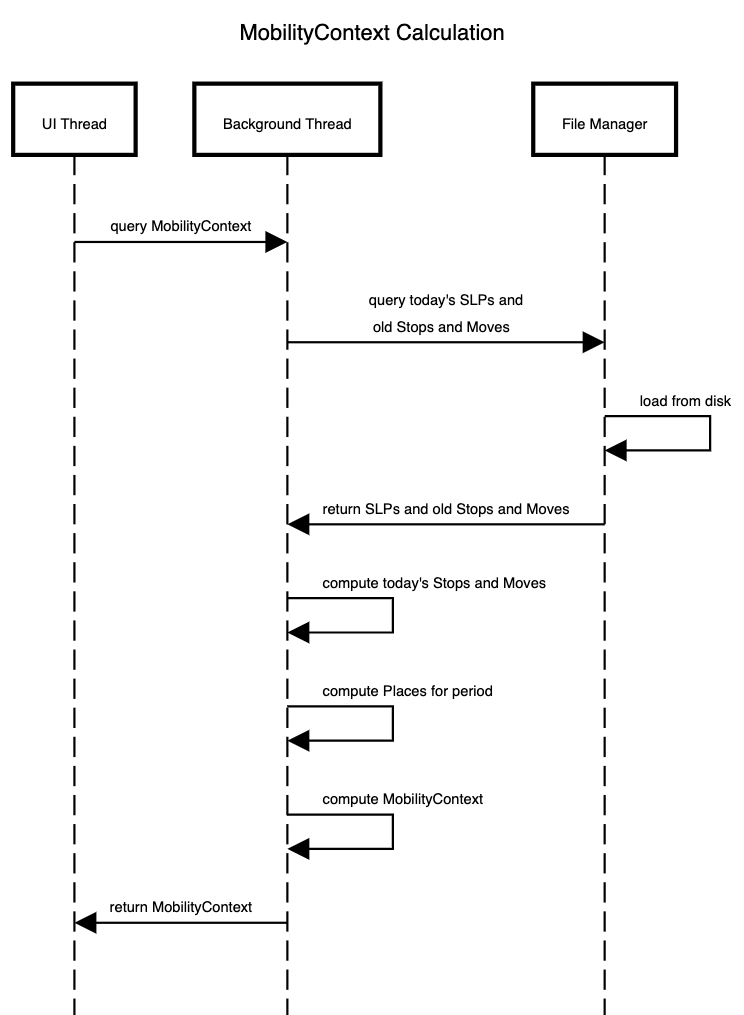
\includegraphics{images/diagrams/sequence.png}
    \caption{Sequence diagram for the computation of the Mobility Context in a Flutter application}
    \label{fig:sequence-diagram-mobility-context}
\end{figure}